\documentclass[hyperref={pdfpagelabel=false},usepdftitle=false,xcolor=dvipsnames]{beamer}

\usepackage[T3]{fontenc}
\usepackage[utf8]{inputenc}
\usepackage[russian]{babel}

\usepackage{mhchem}
\usepackage{amssymb, amsmath}

\usepackage{tikz}
\usetikzlibrary{shapes.geometric, arrows, positioning, decorations.markings}
\usetikzlibrary{fit}
\usepackage{microtype}
\usepackage{framed}
\usetikzlibrary{decorations.pathmorphing,calc,backgrounds}

\usepackage{animate}

\usepackage{fixltx2e}
\usepackage{hyperref}

%\usetheme{Berkeley}
%\usetheme{Madrid} -- неплохо
%\usetheme{CambridgeUS}
%\usetheme{Singapore}
\usetheme{Warsaw}

\pdfmapfile{+sansmathaccent.map}

\title{Исследование бифуркаций в трехатомных гидридах методом классических траекторий}

\author{\small 
Финенко Артем \\[1ex] 
Научный руководитель: Петров С.В.}

\institute[MSU] % (optional, but mostly needed)
{
  МГУ им. М.В.Ломоносова \\
  Химический факультет
}

\date{23/12/2016}

\pgfdeclareimage[height=0.5cm]{university-logo}{../pictures/logo.jpg}
\logo{\pgfuseimage{university-logo}}

\newcommand\Fontvi{\fontsize{6}{7.2}\selectfont}

\beamertemplatenavigationsymbolsempty

\setbeamerfont{page number in head/foot}{size=\large}
\setbeamertemplate{footline}[frame number]
\setbeamertemplate{frametitle}[default][center]

% change font
\usefonttheme[onlymath]{serif}

% custom block environment
\newenvironment<>{varblock}[2][.9\textwidth]{%
  \setlength{\textwidth}{#1}
  \begin{actionenv}#3%
    \def\insertblocktitle{#2}%
    \par%
    \usebeamertemplate{block begin}}
  {\par%
    \usebeamertemplate{block end}%
  \end{actionenv}}

\tikzstyle{lagrange} = [rectangle, rounded corners, minimum width = 3cm, minimum height = 1cm, text centered, text width = 5cm, draw = black, fill=DarkOrchid!40]

\tikzstyle{equations} = [rectangle, rounded corners, text centered, draw = black, fill=green!30]

\tikzstyle{hamilton} = [rectangle, rounded corners, minimum width = 3cm, minimum height = 1cm, text centered, text width = 5 cm, draw = black, fill = Goldenrod!50]

\tikzstyle{result} = [rectangle, rounded corners, text centered, draw = black, fill = blue!30]

\tikzstyle{arrow} = [thick, ->, >=stealth]

\tikzstyle{vecArrow} = [thick, decoration={markings,mark=at position
   1 with {\arrow[semithick]{open triangle 60}}},
   double distance=1.4pt, shorten >= 5.5pt,
   preaction = {decorate},
   postaction = {draw,line width=1.4pt, white,shorten >= 4.5pt}]

\usepackage{caption}
\usepackage{subcaption}

\usepackage{graphicx}

\newcommand{\lb}{\left(}
\newcommand{\rb}{\right)}

\begin{document}

\begin{frame}{\normalsize Резонаторный спектрометр (Cavity Ring-down Experiment)}
\begin{block}{}
\begin{figure}
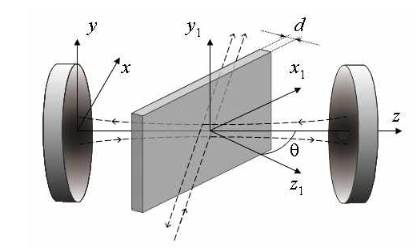
\includegraphics[width = 0.5\linewidth]{pictures/fabry-perot.png}
\caption{\tiny Схема открытого резонатора Фабри-Перо с диэлектрической пленкой связи}
\end{figure}
\end{block}
\begin{block}{}
	\begin{center}
	\scalebox{0.7}{$ \displaystyle Q = \frac{\omega_0 W}{P_d} = \frac{\omega_0}{\Delta \omega} $} \\
	\scalebox{0.7}{$ \displaystyle P = P_{res.} + P_{gas}, \quad P_{gas} = \frac{1}{2} \left( 1 - \exp \left( - 2 \alpha L \right) \right) \approx \alpha L$} \\
	\scalebox{0.7}{\textit{leakage ringdown}: $\displaystyle I = I_0 \exp \lb - \frac{t}{\tau_0} \rb, \quad \tau_0 = \frac{L}{c(1 - R)}$} \\
	\scalebox{0.7}{\textit{absorber presence}: $\displaystyle I = I_0 \exp \lb - \frac{t}{\tau} \rb, \quad A = \frac{L}{c} \lb \frac{1}{\tau} - \frac{1}{\tau_0} \rb$}
	\end{center}
\end{block}
\end{frame}

\begin{frame}{\normalsize CRDS Experimental set-up}
	\begin{figure}
		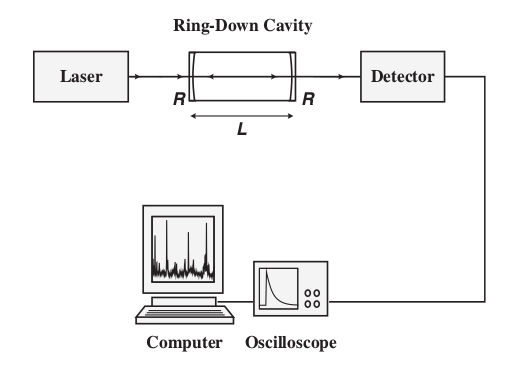
\includegraphics[width = 0.8\linewidth]{pictures/ringdown.png}
	\end{figure}
\end{frame}

\begin{frame}{Столкновительно-индуцированное поглощение}
	\begin{itemize}
		\item Молекулярный и "супермолекулярный" спектр
		\item Столкновение как источник линии поглощения
		\item Аналог вириального разложения для поглощения: \\
			\centering \scalebox{0.8}{$ \alpha = A n + B n^2 + C n^3 + \dots$} \\
\begin{center} A -- dipole allowed contribution, \\ 
	       B -- induced binary contribution, \\
	       C -- induced ternary contribution
\end{center}
			
	\end{itemize}
\end{frame}

\begin{frame}{Бинарный трансляционный спектр}
	\begin{block}{}
		\begin{figure}
			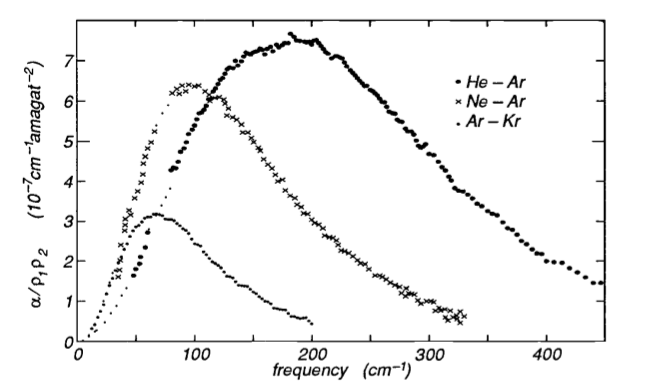
\includegraphics[width = \linewidth]{pictures/trans.png}
		\end{figure}
	\end{block}
\end{frame}

\end{document}
